\documentclass[12pt]{article}

\usepackage{amsmath, mathtools}
\usepackage{amsfonts}
\usepackage{amssymb}
\usepackage{graphicx}
\usepackage{colortbl}
\usepackage{xr}
\usepackage{hyperref}
\usepackage{longtable}
\usepackage{xfrac}
\usepackage{tabularx}
\usepackage{float}
\usepackage{siunitx}
\usepackage{booktabs}
\usepackage{caption}
\usepackage{pdflscape}
\usepackage{afterpage}
\usepackage{placeins}

\usepackage[round]{natbib}

%\usepackage{refcheck}

\hypersetup{
    bookmarks=true,         % show bookmarks bar?
    colorlinks=true,        % false: boxed links; true: colored links
    linkcolor=red,          % color of internal links (change box color with linkbordercolor)
    citecolor=green,        % color of links to bibliography
    filecolor=magenta,      % color of file links
    urlcolor=cyan           % color of external links
}

%% Comments

\usepackage{color}

\newif\ifcomments\commentstrue %displays comments
%\newif\ifcomments\commentsfalse %so that comments do not display

\ifcomments
\newcommand{\authornote}[3]{\textcolor{#1}{[#3 ---#2]}}
\newcommand{\todo}[1]{\textcolor{red}{[TODO: #1]}}
\else
\newcommand{\authornote}[3]{}
\newcommand{\todo}[1]{}
\fi

\newcommand{\wss}[1]{\authornote{blue}{SS}{#1}} 
\newcommand{\plt}[1]{\authornote{magenta}{TPLT}{#1}} %For explanation of the template
\newcommand{\an}[1]{\authornote{cyan}{Author}{#1}}

%% Common Parts

\newcommand{\progname}{Sayyara}
\newcommand{\authname}{Team 3, Tiny Coders
	\\ Arkin Modi
	\\ Joy Xiao
	\\ Leon So
	\\ Timothy Choy} % AUTHOR NAMES

\usepackage{hyperref}
\hypersetup{colorlinks=true, linkcolor=blue, citecolor=blue, filecolor=blue,
	urlcolor=blue, unicode=false}
\urlstyle{same}

\usepackage{parskip}
\usepackage{geometry}
\geometry{a4paper, portrait, margin=1in}


% For easy change of table widths
\newcommand{\colZwidth}{1.0\textwidth}
\newcommand{\colAwidth}{0.13\textwidth}
\newcommand{\colBwidth}{0.82\textwidth}
\newcommand{\colCwidth}{0.1\textwidth}
\newcommand{\colDwidth}{0.05\textwidth}
\newcommand{\colEwidth}{0.8\textwidth}
\newcommand{\colFwidth}{0.17\textwidth}
\newcommand{\colGwidth}{0.5\textwidth}
\newcommand{\colHwidth}{0.28\textwidth}

% Used so that cross-references have a meaningful prefix
\newcounter{defnum} %Definition Number
\newcommand{\dthedefnum}{GD\thedefnum}
\newcommand{\dref}[1]{GD\ref{#1}}
\newcounter{datadefnum} %Data definition Number
\newcommand{\ddthedatadefnum}{DD\thedatadefnum}
\newcommand{\ddref}[1]{DD\ref{#1}}
\newcounter{theorynum} %Theory Number
\newcommand{\tthetheorynum}{T\thetheorynum}
\newcommand{\tref}[1]{T\ref{#1}}
\newcounter{tablenum} %Table Number
\newcommand{\tbthetablenum}{T\thetablenum}
\newcommand{\tbref}[1]{TB\ref{#1}}
\newcounter{assumpnum} %Assumption Number
\newcommand{\atheassumpnum}{P\theassumpnum}
\newcommand{\aref}[1]{A\ref{#1}}
\newcounter{goalnum} %Goal Number
\newcommand{\gthegoalnum}{P\thegoalnum}
\newcommand{\gsref}[1]{GS\ref{#1}}
\newcounter{instnum} %Instance Number
\newcommand{\itheinstnum}{IM\theinstnum}
\newcommand{\iref}[1]{IM\ref{#1}}
\newcounter{reqnum} %Requirement Number
\newcommand{\rthereqnum}{P\thereqnum}
\newcommand{\rref}[1]{R\ref{#1}}
\newcounter{nfrnum} %NFR Number
\newcommand{\rthenfrnum}{NFR\thenfrnum}
\newcommand{\nfrref}[1]{NFR\ref{#1}}
\newcounter{lcnum} %Likely change number
\newcommand{\lthelcnum}{LC\thelcnum}
\newcommand{\lcref}[1]{LC\ref{#1}}

\usepackage{fullpage}

\newcommand{\deftheory}[9][Not Applicable]
{
\newpage
\noindent \rule{\textwidth}{0.5mm}

\paragraph{RefName: } \textbf{#2} \phantomsection 
\label{#2}

\paragraph{Label:} #3

\noindent \rule{\textwidth}{0.5mm}

\paragraph{Equation:}

#4

\paragraph{Description:}

#5

\paragraph{Notes:}

#6

\paragraph{Source:}

#7

\paragraph{Ref.\ By:}

#8

\paragraph{Preconditions for \hyperref[#2]{#2}:}
\label{#2_precond}

#9

\paragraph{Derivation for \hyperref[#2]{#2}:}
\label{#2_deriv}

#1

\noindent \rule{\textwidth}{0.5mm}

}

\begin{document}

\title{Software Requirements Specification for \progname: subtitle describing software}
\author{\authname}
\date{\today}

\maketitle

~\newpage

\pagenumbering{roman}

\tableofcontents

~\newpage

\begin{table}[hp]
	\caption{Revision History} \label{TblRevisionHistory}
	\begin{tabularx}{\textwidth}{llX}
		\toprule
		\textbf{Date}      & \textbf{Developer(s)} & \textbf{Change}                                                                    \\
		\midrule
		September 30, 2022 & Leon So               & Add purpose of project                                                             \\
		September 30, 2022 & Joy Xiao              & Add stakeholders                                                                   \\
		September 30, 2022 & Leon So               & Add functional requirements for authentication                                     \\
		September 30, 2022 & Arkin Modi            & Add open issues and new problems sections (effects on the current environment)     \\
		October 1, 2022    & Arkin Modi            & Add user documentation and training, waiting room and ideas for solutions sections \\
		October 1, 2022    & Arkin Modi            & Add project planning, migration to the new product, risks, and costs sections      \\
		October 2, 2022    & Leon So               & Add current situation and appointment diagram                                      \\
		October 2, 2022    & Joy Xiao              & Add current situation quote and invitation diagram                                 \\
		October 3, 2022    & Leon So               & Add current situation work order diagram                                           \\
		October 3, 2022    & Arkin Modi            & Add planning of the development phases and new problems sections                   \\
		October 3, 2022    & Arkin Modi            & Add off-the-shelf solutions sections                                               \\
		October 3, 2022    & Arkin Modi            & Update project title                                                               \\
		\bottomrule
	\end{tabularx}
\end{table}

\newpage

\pagenumbering{arabic}

This document describes the requirements for Sayyara. The template for the Software Requirements
Specification (SRS) is a subset of the Volere template~\citep{RobertsonAndRobertson2012}. If you
make further modifications to the template, you should explicitly state what modifications were
made.

\section{Project Drivers}

\subsection{The Purpose of the Project}

Independent auto repair shops do not have an efficient way of reaching and interacting with new
customers. Currently, many independent shop owners rely on word-of-mouth referrals as a main
channel to acquiring new customers. Independent auto repair shops are also spending a significant
amount of their time on administrative work such as managing appointments and providing quotes. As
a result, independent auto repair shops have a difficult time competing with larger repair shops
which have dedicated systems and services in place.

On the other hand, customers do not have an effective way to find and compare auto repair shops.
Currently, one of the only ways to compare repair shops is by manually searching or reaching out to
repair shops one-by-one. This process can often be repetitive and time-consuming.

Sayyara is a progressive web application (PWA) which will act as a single platform for independent
auto repair shops and vehicle owners. This platform will allow independent auto repair shops and
vehicle owners to interact in a more efficient and effective manner. Vehicle owners can search for
auto repair shops and services based on a variety of search filters; request quotes for service;
book, view, and manage service appointments. On the application, auto repair shop owners will have
full shop management capabilities such as: adding and managing a list of employees; managing a list
of service types and corresponding service appointment availabilities; managing store information
such as location, hours of operation, and contact information. Auto repair shop owners and
employees will be able to manage quotes, service appointments, and work orders from a single
application. Ultimately, Sayyara will significantly improve the auto repair experience for both
independent auto repair shops and vehicle owners.

\subsection{The Stakeholders}

\subsubsection{The Client}
The client of the project is Nabeel Ibrahim. Nabeel will be the point of contact throughout the
development of the project.

\subsubsection{The Customers}
The customers of Sayyara will be independent auto repair shop owners, shop employees, and vehicle
owners who are looking for a vehicle repair or maintenance service.

\subsubsection{Other Stakeholders}
Other stakeholders of the project are the developers, Tiny Coders, who are designing and
implementing the project.

\subsection{Mandated Constraints}

\subsection{Naming Conventions and Terminology}

\subsection{Relevant Facts and Assumptions}

User characteristics should go under assumptions.

\section{Functional Requirements}

\subsection{The Scope of the Work and the Product}

\subsubsection{The Current Situation}
The current interactions between independent auto repair shop owners, employees, and customers
(i.e., vehicle owners), are often a manual process. Outlined below are models for interactions
between the independent auto repair shop owners, employees, customers, and the proposed system.
\begin{figure}[!hbp]
	\centering
	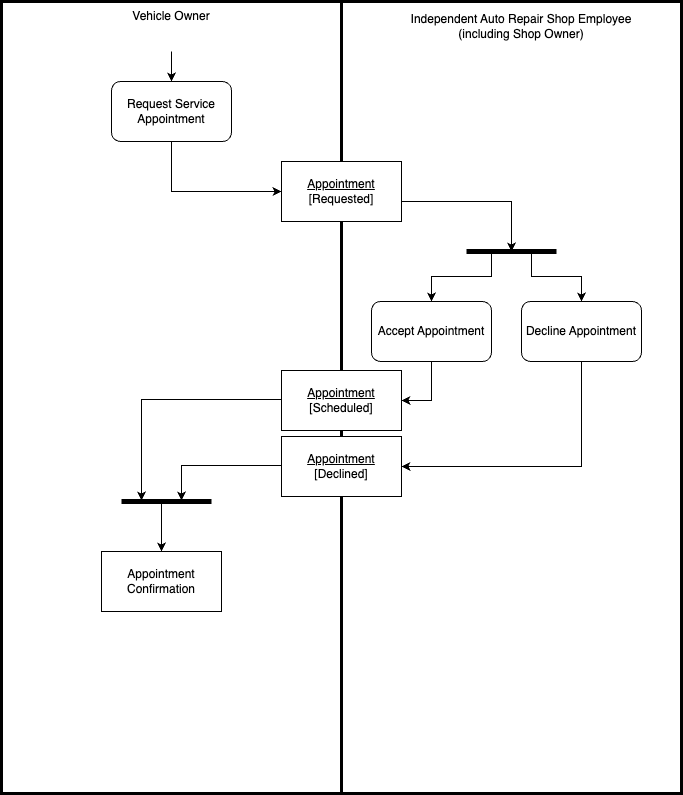
\includegraphics[width=\linewidth/2]{./diagrams/Appointments.png}
	\caption{Service Appointments}
\end{figure}
\FloatBarrier
\begin{figure}[!hbp]
	\centering
	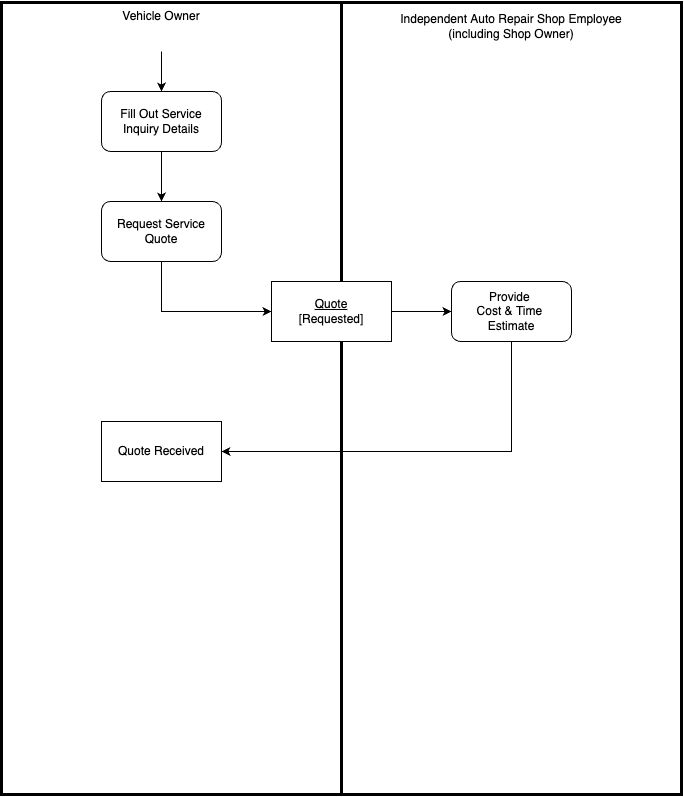
\includegraphics[width=\linewidth/2]{./diagrams/Quotes.png}
	\caption{Service Quotes}
\end{figure}
\FloatBarrier
\begin{figure}[!hbp]
	\centering
	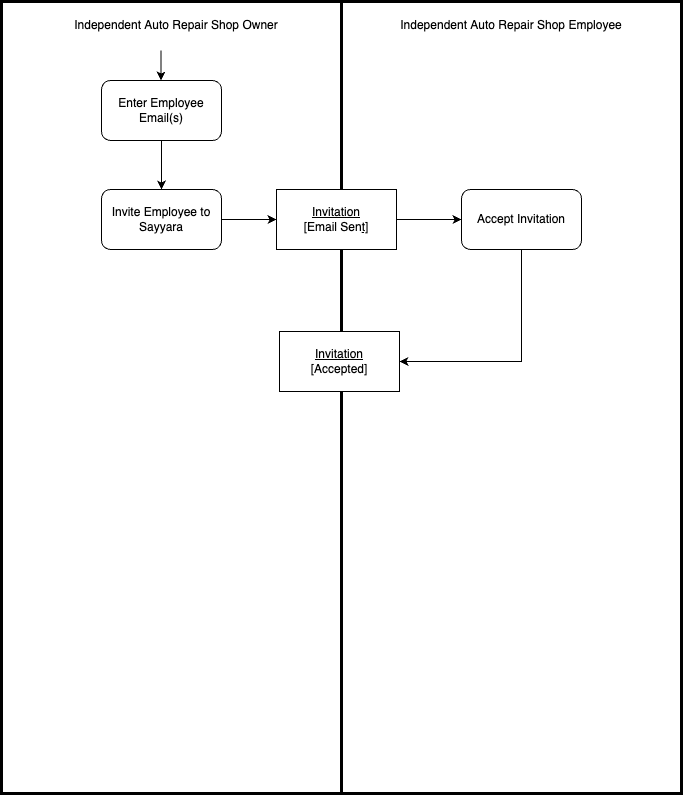
\includegraphics[width=\linewidth/2]{./diagrams/Invitation.png}
	\caption{Employee Invitation to Join Auto Repair Shop}
\end{figure}
\FloatBarrier
\begin{figure}[!hbp]
	\centering
	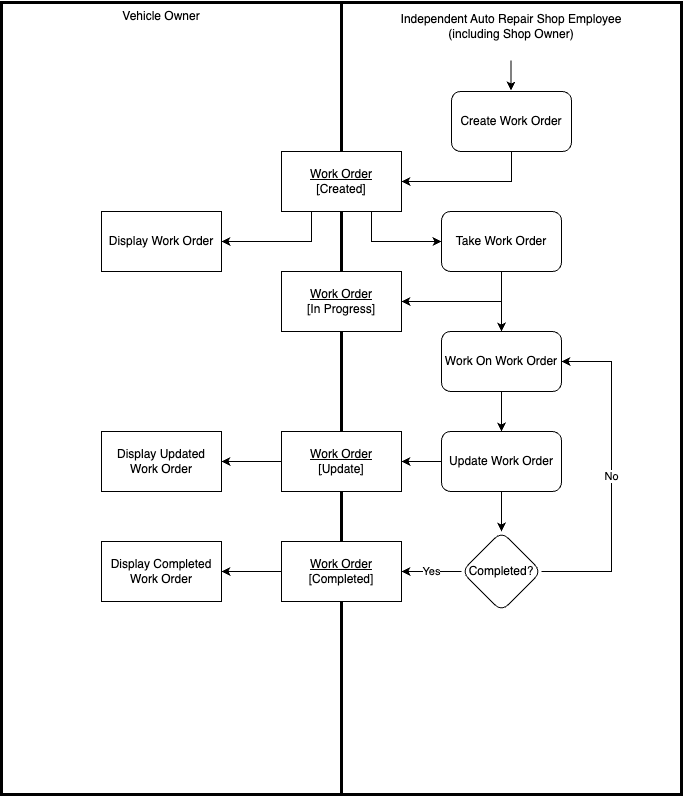
\includegraphics[width=\linewidth/2]{./diagrams/WorkOrder.png}
	\caption{Work Orders}
\end{figure}
\FloatBarrier

\subsubsection{Work Partitioning}

\subsubsection{Individual Product Use Cases}

\subsection{Functional Requirements}
\subsubsection{Authentication}
\begin{enumerate}
	\item [{BE}1.] The user wants to sign up for an account
	      \begin{enumerate}
		      \item [{VP1}.1] Viewpoint: Vehicle Owner
		            \begin{enumerate}
			            \item The system shall allow the user to enter an email and password
			            \item The system shall allow the user to enter their name
			            \item The system shall allow the user to enter their phone number
			            \item The system shall transition to the vehicle owner landing page after the registration process is
			                  complete and successful
			            \item The system shall allow the user to cancel and exit the registration process
		            \end{enumerate}
	      \end{enumerate}
	      \begin{enumerate}
		      \item [{VP1}.2] Viewpoint: Auto Repair Shop Owner
		            \begin{enumerate}
			            \item The system shall allow the user to enter an email and password
			            \item The system shall allow the user to enter their name
			            \item The system shall allow the user to enter their phone number
			            \item The system shall allow the user to enter the shop name
			            \item The system shall allow the user to enter the shop address
			            \item The system shall allow the user to enter the shop phone number
			            \item The system shall transition to the shop owner landing page after the registration process is
			                  complete and successful
			            \item The system shall allow the user to cancel and exit the registration process
		            \end{enumerate}
	      \end{enumerate}
	      \begin{enumerate}
		      \item [{VP1}.3] Viewpoint: Auto Repair Shop Employee
		            \begin{enumerate}
			            \item The system shall allow the user to enter an email and password
			            \item The system shall allow the user to enter their name
			            \item The system shall allow the user to enter their phone number
			            \item The system shall transition to the employee landing page after the registration process is complete
			                  and successful
			            \item The system shall allow the user to cancel and exit the registration process
		            \end{enumerate}
	      \end{enumerate}
\end{enumerate}

\begin{enumerate}
	\item [{BE}2.] The user wants to login to their account
	      \begin{enumerate}
		      \item [{VP1}.1] Viewpoint: Vehicle Owner
		            \begin{enumerate}
			            \item The system shall allow the user to enter their email and password
			            \item The system shall transition to the vehicle owner landing page after the login process is complete
			                  and successful
			            \item The system shall allow the user to cancel and exit the login process
		            \end{enumerate}
	      \end{enumerate}
	      \begin{enumerate}
		      \item [{VP1}.2] Viewpoint: Auto Repair Shop Owner
		            \begin{enumerate}
			            \item The system shall allow the user to enter their email and password
			            \item The system shall transition to the shop owner landing page after the login process is complete and
			                  successful
			            \item The system shall allow the user to cancel and exit the login process
		            \end{enumerate}
	      \end{enumerate}
	      \begin{enumerate}
		      \item [{VP1}.3] Viewpoint: Auto Repair Shop Employee
		            \begin{enumerate}
			            \item The system shall allow the user to enter their email and password
			            \item The system shall transition to the employee landing page after the login process is complete and
			                  successful
			            \item The system shall allow the user to cancel and exit the login process
		            \end{enumerate}
	      \end{enumerate}
\end{enumerate}

\section{Non-functional Requirements}

\subsection{Look and Feel Requirements}

\subsection{Usability and Humanity Requirements}

\subsection{Performance Requirements}

\subsection{Operational and Environmental Requirements}

\subsection{Maintainability and Support Requirements}

\subsection{Security Requirements}

\subsection{Cultural Requirements}

\subsection{Legal Requirements}

\subsection{Health and Safety Requirements}

This section is not in the original Volere template, but health and safety are issues that should
be considered for every engineering project.

\section{Project Issues}

\subsection{Open Issues}

There are currently no known open issues that may lead to significant change to the product or its
design.

\subsection{Off-the-Shelf Solutions}

\subsubsection{Ready-Made Products}

There are existing services that solve many of the problems that this application aims to fix.
These include AutoLeap (https://autoleap.com), Sayaaraa (https://sayaaraa.com/), and KUKUI
(https://www.kukui.com/). These are all paid services and most offer a trial period.

\subsubsection{Resuable Components}

There are many libraries and frameworks available that can be reused to accelerate the building
process of the application. Next.js can be used to provide a framework in which to build the
application. Next.js comes with many out-of-box solutions for common website development problems.
NextAuth.js is a library designed to help simplify the authentication process. Prisma is a library
designed to help simplify the communication between the application and the database. Next-PWA is a
library designed to quickly bootstrap a Next.js application into a progressive web application.

All libraries and frameworks list above are free to use for private and commercial use.

\subsubsection{Products That Can Be Copied}

There are no known products available that can be legally copied for use in this application.

\subsection{New Problems}

\subsubsection{Effects on the Current Environment}

This application will change the way certain processes are preformed and these changes will impact
the users.

\textbf{Work Orders}

The work order system will affect the way automotive mechanics document their work. The data will
be inputted into the application therefore any failures can result in data loss.

\textbf{Appointments}

The appointments system will affect the way that both the customers and the receptionists schedule
appointments. The application will track daily appointment schedules and report time conflicts. The
application shall not lock the receptionist out of overriding the schedule.

\textbf{Quotes}

The quotes system will affect the way that both the customers and automotive repair shops
communicate quotes. The quotes will now be communicated partially or completely through the
application instead of completely in-person. Failure in this system may lead to a loss in data.

\subsubsection{Effects on the Installed Systems}

The application will be standing completely alone and will not be interfacing with any existing
systems. The existing system may continue to coexist with the application at the user's discretion.

\subsubsection{Potential User Problems}

Any potential adverse reactions to using computer would extend to the use of this application. The
application will not introduce any new adverse reactions to the user.

\subsubsection{Limitations in the Anticipated Implementation Environment That May Inhibit the New Product}

The database is not able to sustain the number of connections to serve all requests.

\subsubsection{Follow-Up Problems}

There are no forseeable follow up problems that may cause the application to fail.

\subsection{Tasks}
\subsubsection{Project Planning}
The project schedule will follow the deadline for the deliverables outlined in the SFWRENG 4G06
course outline.

\begin{table}[H]
	\centering
	\caption{Project Tasks}
	\vspace{5pt}
	\begin{tabular}{|p{0.2\textwidth}|p{0.4\textwidth}|p{0.3\textwidth}|}
		\hline
		\textbf{Phase} & \textbf{Task}                      & \textbf{Due Date}                 \\
		\hline
		Phase 1        & Hazard Analysis                    & October 19, 2022                  \\
		\cline{2-3}    & Verification and Validation Plan   & November 2, 2022                  \\
		\cline{2-3}    & Proof of Concept Demonstration     & November 14, 2022                 \\
		\cline{2-3}    & Design Documentation               & January 18, 2023                  \\
		\cline{2-3}    & Revision 0 Demonstration           & February 6 \textemdash{} 17, 2023 \\
		\hline
		Phase 2        & Verification and Validation Report & March 8, 2023                     \\
		\cline{2-3}    & Final Demonstration                & March 20 \textemdash{} 31, 2023   \\
		\cline{2-3}    & Final Documentation                & April 5, 2023                     \\
		\hline
	\end{tabular}

	\label{project_tasks}
\end{table}

\subsubsection{Planning of the Development Phases}

The development of the project will be conducted in two phases:

\begin{enumerate}
	\item Initial development of application and documentation
	\item Refinement of application and documentation
\end{enumerate}

Phase 1 is where the bulk of the application will be designed and implemented. The design of both
the components of the application and how the components will interact will de developed.
Additional, Phase 1 is where most of the documentation and report will be written. Phase 1 will end
with the Revision 0 Demonstration. Here the stakeholders will see the application implementation
and be able to provide feedback.

Phase 2 will be focused on refining the application and the documentation. There is expected to be
no new major feature development and instead, all efforts will be focused on incorporating the
stakeholders' feedback into the application.

\subsection{Migration to the New Product}
\subsubsection{Requirements for Migration to the New Product}

There are no requirements for migrating to the new product.

\subsubsection{Data That Has to Be Modified or Translated for the New System}

No data needs to be modified or translated to the new system.

\subsection{Risks}

\begin{itemize}
	\item Failures in the work orders and quotes work flow may lead to data loss.
	\item Failures in the appointments work flow may lead to a loss in appointment or conflicting
	      appointments.
	\item Failure to meet deadlines will cause set backs in project's timeline. In the event of this, lower
	      priority requirements may need to be dropped.
\end{itemize}

\subsection{Costs}

There are no financial costs associated with the development of this application. All software and
cloud infrastructure used are free to use. There will be about six months of development time
required.

\subsection{User Documentation and Training}
\subsubsection{User Documentation Requirements}

The application will feature a ``Getting Started'' guide, where it shall guide the user through the
most common use cases. For vehicle owners, the use cases will include: searching for shops,
requesting quotes, and scheduling appointments. For automotive shops, the use cases include:
setting shop details, managing appointments, managing employees, responding to quotes, and managing
work orders.

\subsubsection{Training Requirements}

Knowledge of how to navigate a website will be required. Documentation concerning detailed usage of
the website's user flows will be provided to the user.

\subsection{Waiting Room}

There are currently no requirements that are not part of the initial release.

% todo: could be a good place to put the stretch goals

\subsection{Ideas for Solutions}

% todo: ask the rest of the team on what they would add here

During the requirements collection and understanding phase, some ideas with regard to what tooling
will be used have occurred.

\begin{itemize}
	\item Form
	      \begin{itemize}
		      \item With the constraint of this application to be a PWA, the idea of using a React based framework,
		            specifically Next.js.
	      \end{itemize}
	\item Authentication
	      \begin{itemize}
		      \item To handle authentication, using emails and passwords, with the package NextAuth.js.
		      \item Creating a dedicated endpoint in the backend for looking up user information.
	      \end{itemize}
\end{itemize}

\newpage

\bibliographystyle{plainnat}

\bibliography {../../refs/References}

\newpage

\noindent \plt{The following is not part of the template, just some things to consider
	when filing in the template.}

\noindent \plt{Grammar, flow and \LaTeX advice:
	\begin{itemize}
		\item For Mac users \texttt{*.DS\_Store} should be in \texttt{.gitignore}
		\item \LaTeX{} and formatting rules
		      \begin{itemize}
			      \item Variables are italic, everything else not, includes subscripts (link to document)
			            \begin{itemize}
				            \item \href{https://physics.nist.gov/cuu/pdf/typefaces.pdf}{Conventions}
				            \item Watch out for implied multiplication
			            \end{itemize}
			      \item Use BibTeX
			      \item Use cross-referencing
		      \end{itemize}
		\item Grammar and writing rules
		      \begin{itemize}
			      \item Acronyms expanded on first usage (not just in table of acronyms)
			      \item ``In order to'' should be ``to''
		      \end{itemize}
	\end{itemize}}

\noindent \plt{Advice on using the template:
	\begin{itemize}
		\item Difference between physical and software constraints
		\item Properties of a correct solution means \emph{additional} properties, not a restating of the
		      requirements (may be ``not applicable'' for your problem). If you have a table of output
		      constraints, then these are properties of a correct solution.
		\item Assumptions have to be invoked somewhere
		\item ``Referenced by'' implies that there is an explicit reference
		\item Think of traceability matrix, list of assumption invocations and list of reference by fields as
		      automatically generatable
		\item If you say the format of the output (plot, table etc), then your requirement could be more abstract
	\end{itemize}
}
\section{Appendix}

This section has been added to the Volere template. This is where you can place additional
information.

\newpage{}
\section*{Appendix --- Reflection}

The information in this section will be used to evaluate the team members on the graduate attribute
of Lifelong Learning. Please answer the following questions:

\begin{enumerate}
	\item What knowledge and skills will the team collectively need to acquire to successfully complete this
	      capstone project? Examples of possible knowledge to acquire include domain specific knowledge from
	      the domain of your application, or software engineering knowledge, mechatronics knowledge or
	      computer science knowledge. Skills may be related to technology, or writing, or presentation, or
	      team management, etc. You should look to identify at least one item for each team member.
	\item For each of the knowledge areas and skills identified in the previous question, what are at least
	      two approaches to acquiring the knowledge or mastering the skill? Of the identified approaches,
	      which will each team member pursue, and why did they make this choice?
\end{enumerate}

\subsection{Symbolic Parameters}

The definition of the requirements will likely call for SYMBOLIC\_CONSTANTS. Their values are
defined in this section for easy maintenance.

\end{document}
